

\tikzset{every picture/.style={line width=0.75pt}} %set default line width to 0.75pt        

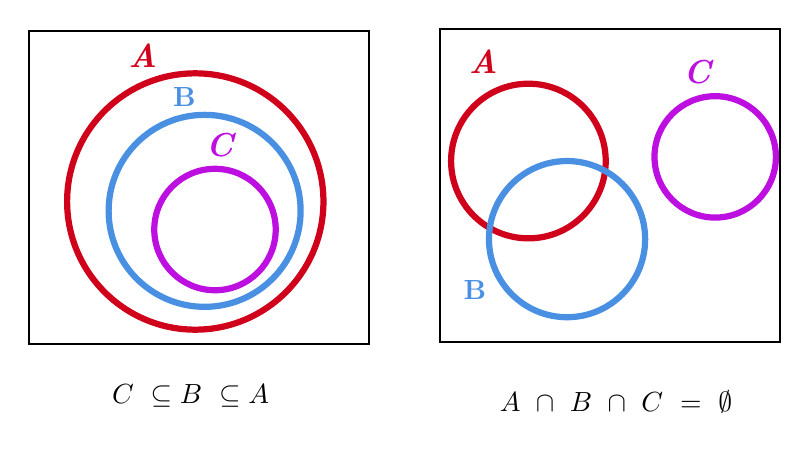
\begin{tikzpicture}[x=0.75pt,y=0.75pt,yscale=-1,xscale=1]
%uncomment if require: \path (0,222); %set diagram left start at 0, and has height of 222

%Shape: Circle [id:dp3347773199535533] 
\draw  [color={rgb, 255:red, 208; green, 2; blue, 27 }  ,draw opacity=1 ][line width=2.25]  (123.5,93.25) .. controls (123.5,59.15) and (151.15,31.5) .. (185.25,31.5) .. controls (219.35,31.5) and (247,59.15) .. (247,93.25) .. controls (247,127.35) and (219.35,155) .. (185.25,155) .. controls (151.15,155) and (123.5,127.35) .. (123.5,93.25) -- cycle ;
%Shape: Circle [id:dp8501218983400187] 
\draw  [color={rgb, 255:red, 74; green, 144; blue, 226 }  ,draw opacity=1 ][line width=2.25]  (143.5,97.75) .. controls (143.5,72.21) and (164.21,51.5) .. (189.75,51.5) .. controls (215.29,51.5) and (236,72.21) .. (236,97.75) .. controls (236,123.29) and (215.29,144) .. (189.75,144) .. controls (164.21,144) and (143.5,123.29) .. (143.5,97.75) -- cycle ;
%Shape: Circle [id:dp028727913020643925] 
\draw  [color={rgb, 255:red, 189; green, 16; blue, 224 }  ,draw opacity=1 ][line width=2.25]  (165.5,106.75) .. controls (165.5,90.6) and (178.6,77.5) .. (194.75,77.5) .. controls (210.9,77.5) and (224,90.6) .. (224,106.75) .. controls (224,122.9) and (210.9,136) .. (194.75,136) .. controls (178.6,136) and (165.5,122.9) .. (165.5,106.75) -- cycle ;
%Shape: Circle [id:dp6019981075283429] 
\draw  [color={rgb, 255:red, 208; green, 2; blue, 27 }  ,draw opacity=1 ][line width=2.25]  (308.5,73.75) .. controls (308.5,53.18) and (325.18,36.5) .. (345.75,36.5) .. controls (366.32,36.5) and (383,53.18) .. (383,73.75) .. controls (383,94.32) and (366.32,111) .. (345.75,111) .. controls (325.18,111) and (308.5,94.32) .. (308.5,73.75) -- cycle ;
%Shape: Circle [id:dp707293905477145] 
\draw  [color={rgb, 255:red, 74; green, 144; blue, 226 }  ,draw opacity=1 ][line width=2.25]  (326.75,111.38) .. controls (326.75,90.6) and (343.6,73.75) .. (364.38,73.75) .. controls (385.15,73.75) and (402,90.6) .. (402,111.38) .. controls (402,132.15) and (385.15,149) .. (364.38,149) .. controls (343.6,149) and (326.75,132.15) .. (326.75,111.38) -- cycle ;
%Shape: Circle [id:dp13160094529110977] 
\draw  [color={rgb, 255:red, 189; green, 16; blue, 224 }  ,draw opacity=1 ][line width=2.25]  (406.5,71.75) .. controls (406.5,55.6) and (419.6,42.5) .. (435.75,42.5) .. controls (451.9,42.5) and (465,55.6) .. (465,71.75) .. controls (465,87.9) and (451.9,101) .. (435.75,101) .. controls (419.6,101) and (406.5,87.9) .. (406.5,71.75) -- cycle ;
%Shape: Rectangle [id:dp4210802571053138] 
\draw   (105,11) -- (269,11) -- (269,162) -- (105,162) -- cycle ;
%Shape: Rectangle [id:dp3258541513105915] 
\draw   (303,10) -- (467,10) -- (467,161) -- (303,161) -- cycle ;

% Text Node
\draw (160,23) node [scale=1,color={rgb, 255:red, 245; green, 166; blue, 35 }  ,opacity=1 ] [align=left] {\textit{\textcolor[rgb]{0.82,0.01,0.11}{{\large \textbf{A}}}}};
% Text Node
\draw (180,43) node [scale=1,color={rgb, 255:red, 80; green, 227; blue, 194 }  ,opacity=1 ] [align=left] {\textcolor[rgb]{0.29,0.56,0.89}{\textbf{B}}};
% Text Node
\draw (197,66) node [scale=1,color={rgb, 255:red, 80; green, 227; blue, 194 }  ,opacity=1 ] [align=left] {{\large \textbf{\textit{\textcolor[rgb]{0.74,0.06,0.88}{C}}}}};
% Text Node
\draw (183,187) node   {$C\ \subseteq B\ \subseteq A$};
% Text Node
\draw (427,31) node [scale=1,color={rgb, 255:red, 80; green, 227; blue, 194 }  ,opacity=1 ] [align=left] {{\large \textbf{\textit{\textcolor[rgb]{0.74,0.06,0.88}{C}}}}};
% Text Node
\draw (320,136) node [scale=1,color={rgb, 255:red, 80; green, 227; blue, 194 }  ,opacity=1 ] [align=left] {\textcolor[rgb]{0.29,0.56,0.89}{\textbf{B}}};
% Text Node
\draw (324,26) node [scale=1,color={rgb, 255:red, 245; green, 166; blue, 35 }  ,opacity=1 ] [align=left] {\textit{\textcolor[rgb]{0.82,0.01,0.11}{{\large \textbf{A}}}}};
% Text Node
\draw (388,190) node   {$A\ \cap \ B\ \cap \ C\ =\ \emptyset $};


\end{tikzpicture}